\documentclass{standalone}
\usepackage{standalone}

\begin{document}
\subsection{Suffix Tree}
The name of the title is enough to tell us that Suffix Tree is has to do with the Suffixes of any string/sequence. Suffix Tree has some advantages over Suffix Trie regarding space consumption. Considering the formal definition of we can state that a Suffix Tree for a sequence {\bf{S}} considering it's length as {\bf {m}} is:
\begin{enumerate}
	\item A rooted tree {\bf {T}} with {\bf {m}} leaves numbered from 1 to {\bf {m}}.
	\item Every internal node of {\bf {T}}, except perhaps the root, has at least two children emanating from it. 
	\item Every edge of {\bf {T}} is labeled with a nonempty substring of {\bf {S}}.
	\item Every edge emanating from a node must have edge-labels starting with unique characters.
	\item For any leaf {\bf \emph{i}}, the concatenation of the edge-labels on the path from the root to the leaf {\bf \emph{i}} exactly represents {\bf {S[i,m]}}, the suffix of {\bf{S}} that starts at position {\bf \emph{i}}.
\end{enumerate}
To construct Suffix Tree, we first have to add the terminal character \$ at the end of the text.
For example Suffix Tree for the sequence ATATACA\$ is in figure \ref{fig:ST}\footnote{Generated from https://visualgo.net/suffixtree}
\begin{figure}[ht]
	\centering
	\fbox{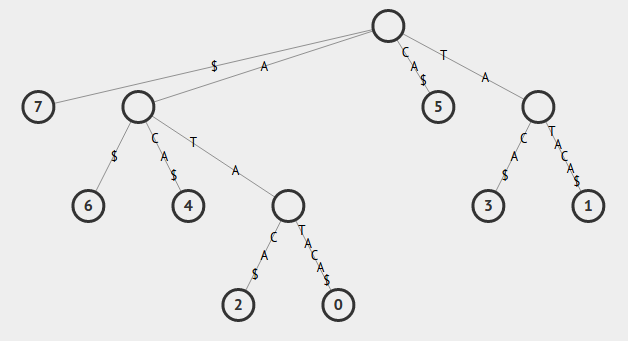
\includegraphics[scale=0.6]{./img/ST}}
	\caption{Suffix Tree for the sequence ATATACA\$.}
	\label{fig:ST}
\end{figure} 

\subsubsection{Analysis}
By constructing the Suffix Tree in the previous example we can obviously perceive that this construction algorithm takes {\bf \emph{O($m^2$)}} time. This can be done in {\bf \emph{O(m)}} time by Ukkonen's Algorithm\cite{STUKO} with a space complexity of {\bf \emph{O(m)}}.
\subsubsection{Real life Application of Suffix Tree}
For gnomic studies in real life, many real life analysis tools uses Suffix Trees as their core level data structure enabling them fast and accurate analysis capability. Some of them enlisted below.
\begin{enumerate}
	\item MUMmer for alignment purpose. \cite{MUMmer1, MUMmer2, MUMmer3}
	\item REPuter for calculating and finding repeats in the whole genome sequence. \cite{REPuter}
	\item Identifying sequence motifs.\cite{MOTIF1, MOTIF2}
	\item Multiple alignment.\cite{MALIGN}
\end{enumerate}
\end{document}